\section{Landasan Teori}

Landasan teori pada bagian ini membahas konsep yang digunakan untuk memahami rancangan sistem \textit{checkout} otomatis Nasi Padang. Pembahasan mencakup \textit{Computer Vision} dan citra digital, \textit{instance segmentation}, YOLO11-seg, penghitungan instans, kalkulasi harga berbasis harga tetap, serta evaluasi kinerja model dan sistem. Detail mengenai dataset, konfigurasi pelatihan, perangkat, dan prosedur pengujian dibahas pada Bab III.

\input{chapters/subchapters/2/2-3-1}
\input{chapters/subchapters/2/2-3-2}
\subsection{YOLO11-seg}

YOLO11-seg merupakan varian YOLO11 yang mendukung tugas \textit{instance segmentation}. Model ini digunakan untuk menghasilkan prediksi lokasi objek, kelas, dan \textit{segmentation mask} dalam satu model sehingga proses klasifikasi lauk dan segmentasi tidak memerlukan dua model yang terpisah \cite{khanam2024,qiu2025}.

\subsubsection*{a. Arsitektur YOLO11-seg}

Diagram arsitektur YOLO11-seg memperlihatkan tiga bagian utama, yaitu \textit{backbone}, \textit{neck}, dan \textit{segmentation head}. Aliran pemrosesan dimulai dari citra masukan pada sisi kiri diagram, dilanjutkan dengan ekstraksi dan penggabungan fitur, kemudian berakhir pada tiga blok \textit{Segment}. Secara ringkas, \textit{backbone} bertugas mengekstraksi fitur dari citra, \textit{neck} menggabungkan fitur pada beberapa skala, dan \textit{segmentation head} menghasilkan informasi kelas, lokasi objek, serta segmentasi untuk setiap instans \cite{khanam2024,qiu2025}.

\begin{figure}[H]
    \centering
    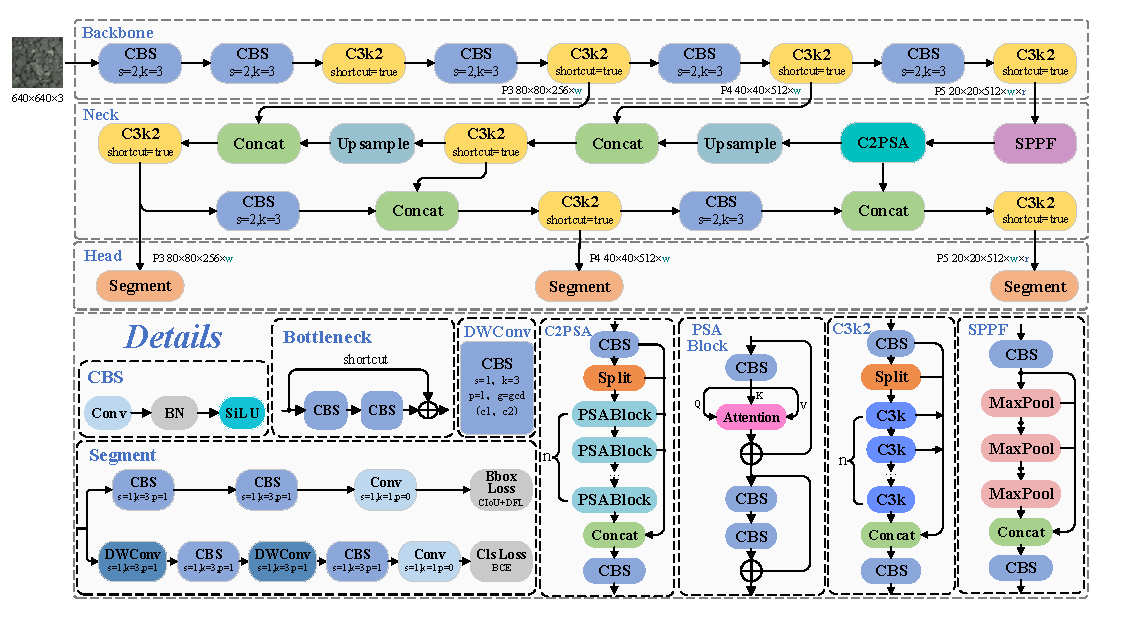
\includegraphics[width=\textwidth]{figures/yolo11-seg-architecture}
    \caption{Arsitektur YOLO11-seg}
    \label{fig:arsitektur-yolo11-seg}
    \par\smallskip
    {\footnotesize Sumber: \cite{qiu2025}}
\end{figure}

\noindent\textbf{\textit{Backbone}.}
Pada bagian paling kiri diagram, citra masukan diproses secara bertahap melalui rangkaian modul CBS dan C3k2. CBS terdiri atas operasi konvolusi, \textit{batch normalization}, dan fungsi aktivasi SiLU, sedangkan C3k2 digunakan untuk melanjutkan proses ekstraksi fitur secara efisien. Setelah melewati beberapa tahapan tersebut, fitur diproses oleh SPPF (\textit{Spatial Pyramid Pooling--Fast}) untuk mengumpulkan informasi konteks melalui operasi \textit{pooling} pada beberapa cakupan. Bagian akhir \textit{backbone} memuat modul C2PSA yang menggunakan mekanisme perhatian untuk menekankan informasi fitur yang relevan. Susunan pada diagram juga menunjukkan bahwa ukuran spasial fitur semakin mengecil pada tahapan yang lebih dalam, sementara informasi yang dibawa fitur menjadi semakin kaya \cite{khanam2024,qiu2025}.

% Aktifkan blok berikut setelah gambar close-up backbone tersedia.
% Jika gambar dipotong dari diagram asli, gunakan keterangan ``Diadaptasi dari''.
% \begin{figure}[H]
%     \centering
%     \includegraphics[width=0.9\textwidth]{figures/yolo11-seg-backbone}
%     \caption{Bagian \textit{backbone} pada arsitektur YOLO11-seg}
%     \label{fig:backbone-yolo11-seg}
%     \par\smallskip
%     {\footnotesize Sumber: Diadaptasi dari \cite{qiu2025}}
% \end{figure}

\noindent\textbf{\textit{Neck}.}
Bagian tengah diagram memperlihatkan bahwa fitur dari beberapa tingkat \textit{backbone} tidak langsung diteruskan ke keluaran. Fitur tersebut terlebih dahulu diproses melalui operasi \textit{upsample}, \textit{concat}, CBS, dan C3k2. Operasi \textit{upsample} memperbesar resolusi peta fitur, sedangkan \textit{concat} menggabungkan fitur tersebut dengan fitur dari tahapan lain. Jalur penggabungan berlangsung dari fitur yang lebih dalam menuju fitur beresolusi lebih tinggi dan kemudian kembali menuju fitur beresolusi lebih rendah. Dengan susunan tersebut, \textit{neck} memadukan detail spasial dari fitur beresolusi tinggi dengan informasi semantik dari fitur yang lebih dalam. Hasilnya adalah tiga tingkat fitur, yaitu P3, P4, dan P5, yang diteruskan ke bagian keluaran \cite{khanam2024,qiu2025}.

% Aktifkan blok berikut setelah gambar close-up neck tersedia.
% \begin{figure}[H]
%     \centering
%     \includegraphics[width=0.9\textwidth]{figures/yolo11-seg-neck}
%     \caption{Penggabungan fitur pada bagian \textit{neck} YOLO11-seg}
%     \label{fig:neck-yolo11-seg}
%     \par\smallskip
%     {\footnotesize Sumber: Diadaptasi dari \cite{qiu2025}}
% \end{figure}

\noindent\textbf{\textit{Segmentation head}.}
Pada bagian kanan diagram, fitur P3, P4, dan P5 masing-masing terhubung dengan satu blok \textit{Segment}. Ketiga tingkat fitur tersebut memungkinkan model melakukan prediksi terhadap objek dengan ukuran yang berbeda. Setiap blok \textit{Segment} menghasilkan informasi yang diperlukan untuk memprediksi kelas objek, posisi \textit{bounding box}, dan segmentasi instans. Dengan demikian, klasifikasi lauk, penentuan lokasi objek, dan segmentasi tidak dilakukan oleh tiga model yang terpisah, tetapi dihasilkan dari fitur bersama dalam satu arsitektur YOLO11-seg \cite{qiu2025}.

% Aktifkan blok berikut setelah gambar close-up segmentation head tersedia.
% \begin{figure}[H]
%     \centering
%     \includegraphics[width=0.9\textwidth]{figures/yolo11-seg-head}
%     \caption{Bagian \textit{segmentation head} pada arsitektur YOLO11-seg}
%     \label{fig:head-yolo11-seg}
%     \par\smallskip
%     {\footnotesize Sumber: Diadaptasi dari \cite{qiu2025}}
% \end{figure}

Mekanisme pembentukan \textit{mask} pada bagian keluaran mengikuti konsep dua cabang. Cabang pertama menghasilkan prediksi kelas, koordinat \textit{bounding box}, dan koefisien \textit{mask} untuk setiap kandidat objek. Cabang kedua menghasilkan sekumpulan \textit{prototype mask} yang digunakan bersama. Koefisien \textit{mask} dari suatu objek kemudian dikombinasikan dengan \textit{prototype mask} untuk membentuk \textit{mask} khusus bagi instans tersebut. Oleh karena itu, dua objek dengan kelas yang sama tetap dapat memperoleh \textit{mask} yang berbeda dan dihitung sebagai dua instans terpisah \cite{qiu2025}.

% Diagram utama tidak memperlihatkan proses pembentukan mask secara terperinci.
% Gambar berikut sebaiknya dibuat ulang sebagai diagram sederhana yang menunjukkan
% alur prototype mask + koefisien mask -> mask setiap instans.
% \begin{figure}[H]
%     \centering
%     \includegraphics[width=0.8\textwidth]{figures/yolo11-seg-mask-formation}
%     \caption{Mekanisme pembentukan \textit{mask} setiap instans pada YOLO11-seg}
%     \label{fig:pembentukan-mask-yolo11-seg}
%     \par\smallskip
%     {\footnotesize Sumber: Diadaptasi dari \cite{qiu2025}}
% \end{figure}

Melalui alur tersebut, satu citra dapat menghasilkan sejumlah prediksi instans yang masing-masing memiliki kelas, lokasi, dan \textit{mask}. Dalam penelitian ini, kelas hasil prediksi digunakan untuk menentukan jenis lauk, sedangkan jumlah instans pada setiap kelas digunakan dalam proses kalkulasi harga.

\subsubsection*{b. Pelatihan YOLO11-seg}

Pelatihan model dapat dimulai dari bobot pralatih agar fitur visual yang telah dipelajari sebelumnya dapat digunakan sebagai titik awal dan kemudian disesuaikan dengan kelas pada dataset penelitian. Pada penelitian ini, bobot YOLO11-seg disesuaikan untuk mengenali sembilan kelas, yaitu nasi, rendang, ayam goreng, perkedel, sayur nangka, daun singkong, telur dadar, telur kari, dan sambal.

Pada proses pelatihan, citra dan \textit{ground truth} diberikan kepada model untuk menghasilkan prediksi lokasi objek, kelas, dan segmentasi. Prediksi tersebut dibandingkan dengan \textit{ground truth} untuk memperoleh nilai \textit{loss}. Nilai \textit{loss} kemudian digunakan dalam proses \textit{backpropagation} untuk memperbarui bobot model secara berulang. Data validasi digunakan untuk memantau performa model selama pelatihan, sedangkan data pengujian digunakan setelah model akhir diperoleh.

Nilai parameter pelatihan, seperti varian YOLO11-seg, ukuran citra masukan, jumlah \textit{epoch}, \textit{batch size}, konfigurasi augmentasi, dan parameter lain yang digunakan pada implementasi dijelaskan pada Bab III.

\input{chapters/subchapters/2/2-3-4}
\input{chapters/subchapters/2/2-3-5}
\input{chapters/subchapters/2/2-3-6}
